\documentclass{standalone}
\usepackage{tikz}
\usetikzlibrary{patterns, positioning}
\usepackage[sfdefault]{ClearSans} %% option 'sfdefault' activates Clear Sans as the default text font
\usepackage[T1]{fontenc}

\begin{document}
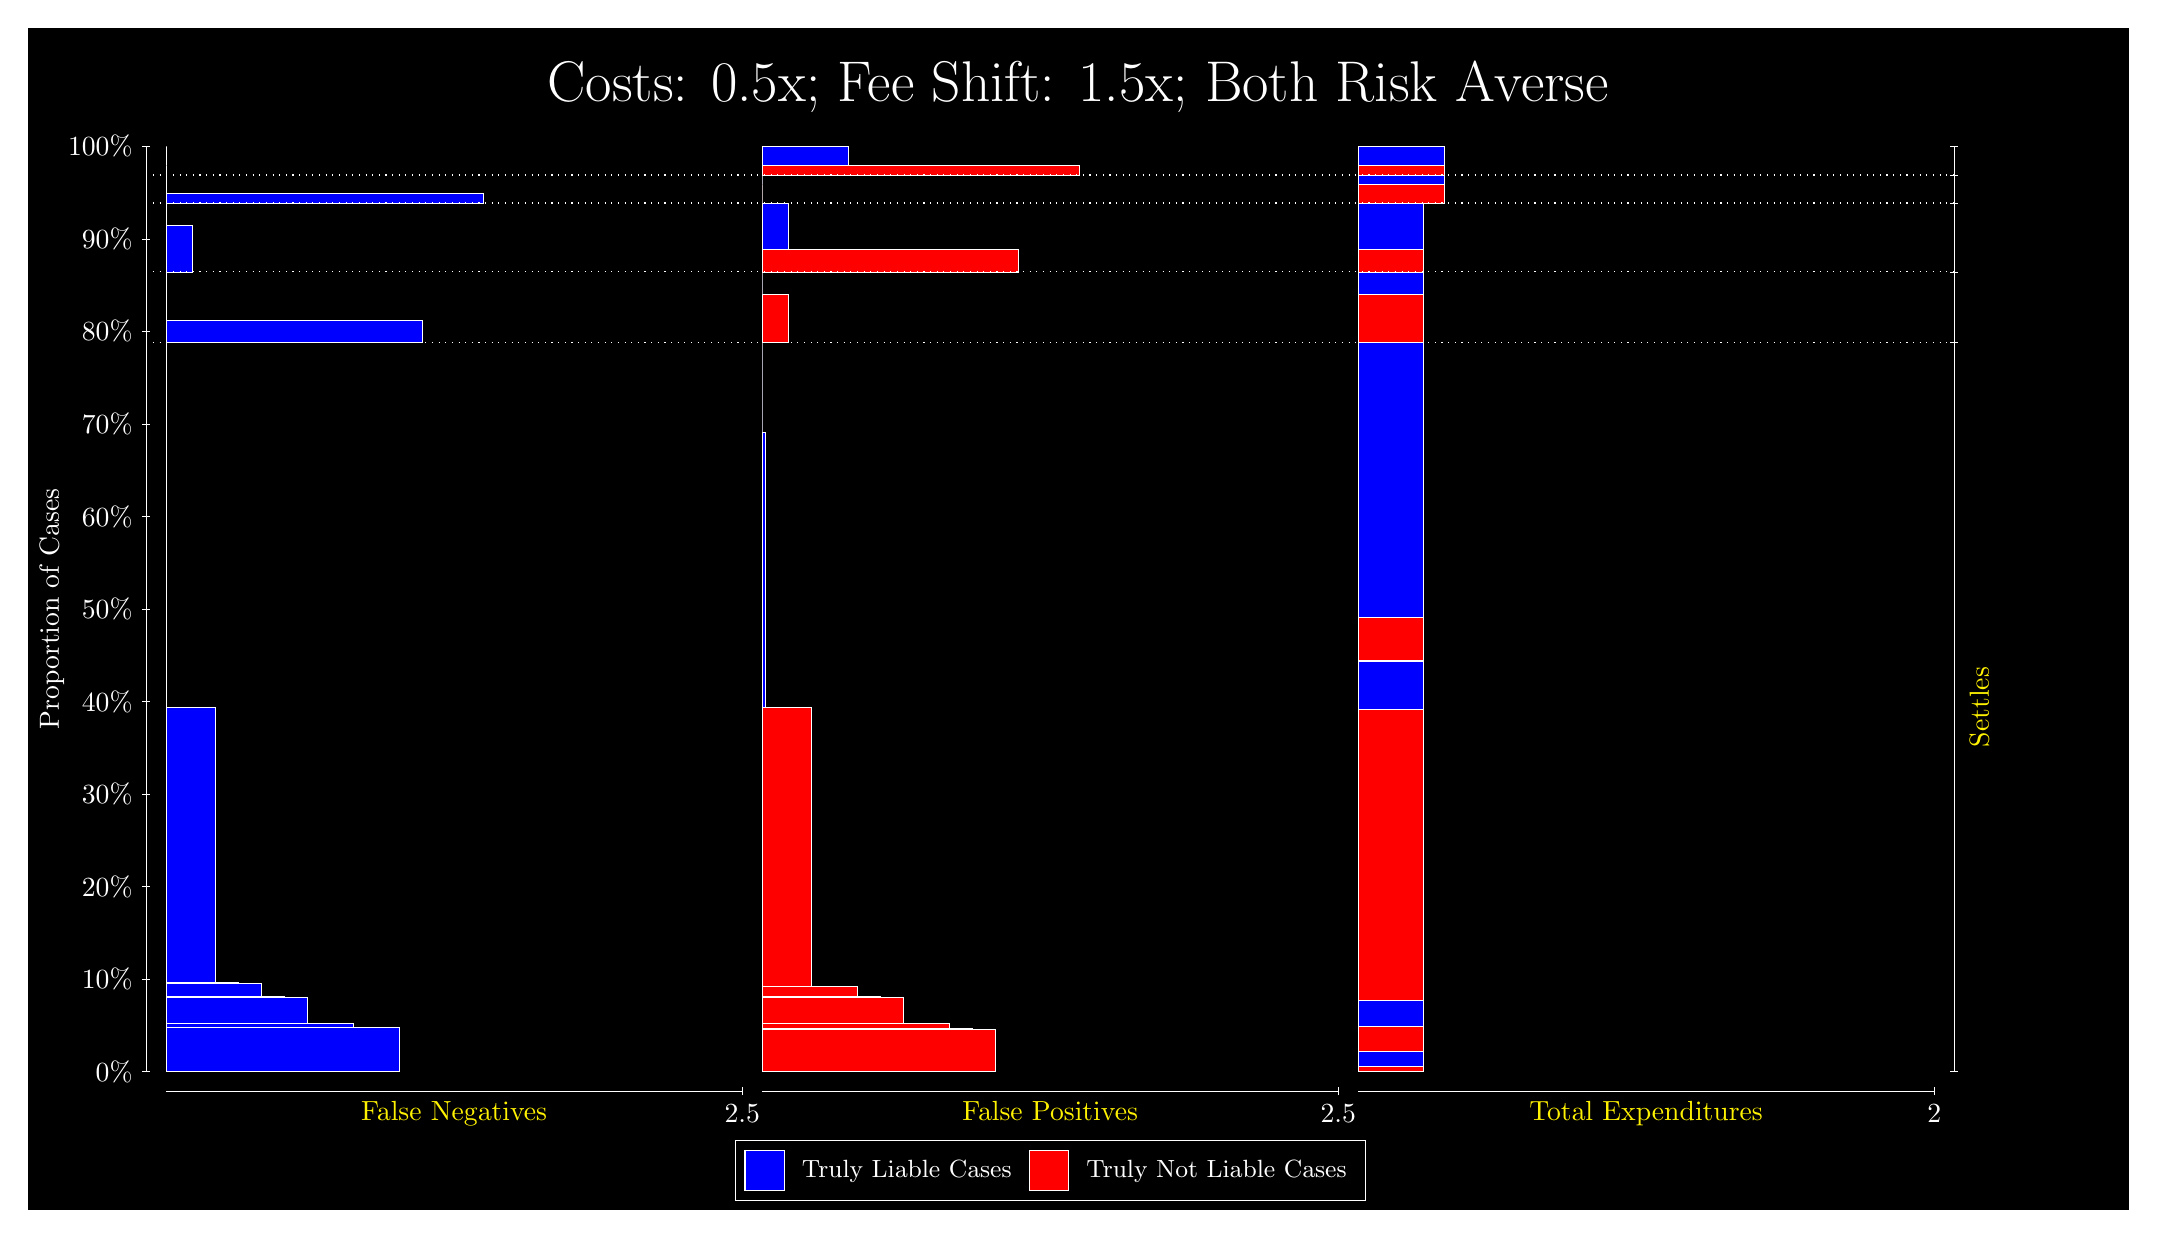
\begin{tikzpicture}
\draw[fill=black] (0,0) rectangle (26.667,15);
\draw[text=white] (0,13.5) rectangle (26.667,15) node[midway] {\huge Costs: 0.5x; Fee Shift: 1.5x; Both Risk Averse};
\draw[white, very thin] (1.5,1.75) -- (1.5,13.5);
\node[rotate=90, text=white, anchor=center] at (0.3, 7.625) {Proportion of Cases};
\draw[white, very thin] (1.45,1.75) -- (1.55,1.75);
\node[text=white, anchor=east] at (1.45, 1.75) {0\%};
\draw[white, very thin] (1.45,2.925) -- (1.55,2.925);
\node[text=white, anchor=east] at (1.45, 2.925) {10\%};
\draw[white, very thin] (1.45,4.1) -- (1.55,4.1);
\node[text=white, anchor=east] at (1.45, 4.1) {20\%};
\draw[white, very thin] (1.45,5.275) -- (1.55,5.275);
\node[text=white, anchor=east] at (1.45, 5.275) {30\%};
\draw[white, very thin] (1.45,6.45) -- (1.55,6.45);
\node[text=white, anchor=east] at (1.45, 6.45) {40\%};
\draw[white, very thin] (1.45,7.625) -- (1.55,7.625);
\node[text=white, anchor=east] at (1.45, 7.625) {50\%};
\draw[white, very thin] (1.45,8.8) -- (1.55,8.8);
\node[text=white, anchor=east] at (1.45, 8.8) {60\%};
\draw[white, very thin] (1.45,9.975) -- (1.55,9.975);
\node[text=white, anchor=east] at (1.45, 9.975) {70\%};
\draw[white, very thin] (1.45,11.15) -- (1.55,11.15);
\node[text=white, anchor=east] at (1.45, 11.15) {80\%};
\draw[white, very thin] (1.45,12.325) -- (1.55,12.325);
\node[text=white, anchor=east] at (1.45, 12.325) {90\%};
\draw[white, very thin] (1.45,13.5) -- (1.55,13.5);
\node[text=white, anchor=east] at (1.45, 13.5) {100\%};

\draw[white, very thin] (24.457,1.75) -- (24.457,13.5);
\draw[white, very thin] (24.407,1.75) -- (24.507,1.75);
\node[anchor=west] at (24.407, 1.75) {};
\draw[white, very thin] (24.407,11.007) -- (24.507,11.007);
\node[anchor=west] at (24.407, 11.007) {};
\draw[white, very thin] (24.407,11.906) -- (24.507,11.906);
\node[anchor=west] at (24.407, 11.906) {};
\draw[white, very thin] (24.407,12.78) -- (24.507,12.78);
\node[anchor=west] at (24.407, 12.78) {};
\draw[white, very thin] (24.407,13.136) -- (24.507,13.136);
\node[anchor=west] at (24.407, 13.136) {};
\draw[white, very thin] (24.407,13.5) -- (24.507,13.5);
\node[anchor=west] at (24.407, 13.5) {};

\draw[white, very thin, fill=blue] (1.75,1.75) rectangle (4.7141,2.3099);
\draw[white, very thin, fill=blue] (1.75,2.3099) rectangle (4.4214,2.3138);
\draw[white, very thin, fill=blue] (1.75,2.3138) rectangle (4.1286,2.3608);
\draw[white, very thin, fill=blue] (1.75,2.3608) rectangle (3.8359,2.3659);
\draw[white, very thin, fill=blue] (1.75,2.3659) rectangle (3.8359,2.3667);
\draw[white, very thin, fill=blue] (1.75,2.3667) rectangle (3.5431,2.6944);
\draw[white, very thin, fill=blue] (1.75,2.6944) rectangle (3.2504,2.7053);
\draw[white, very thin, fill=blue] (1.75,2.7053) rectangle (2.9576,2.8768);
\draw[white, very thin, fill=blue] (1.75,2.8768) rectangle (2.6649,2.8893);
\draw[white, very thin, fill=blue] (1.75,2.8893) rectangle (2.3721,6.3775);
\draw[white, very thin, fill=red] (1.75,6.3775) rectangle (1.75,11.007);
\draw[white, very thin, fill=blue] (1.75,11.007) rectangle (5.0069,11.297);
\draw[white, very thin, fill=red] (1.75,11.297) rectangle (1.75,11.906);
\draw[white, very thin, fill=blue] (1.75,11.906) rectangle (2.0793,12.498);
\draw[white, very thin, fill=red] (1.75,12.498) rectangle (1.75,12.78);
\draw[white, very thin, fill=blue] (1.75,12.78) rectangle (5.7754,12.899);
\draw[white, very thin, fill=red] (1.75,12.899) rectangle (1.75,13.136);
\draw[white, very thin, fill=red] (1.75,13.136) rectangle (1.75,13.254);
\draw[white, very thin, fill=blue] (1.75,13.254) rectangle (1.75,13.5);
\draw[white, very thin, fill=red] (9.3189,1.75) rectangle (12.283,2.2893);
\draw[white, very thin, fill=red] (9.3189,2.2893) rectangle (11.99,2.2941);
\draw[white, very thin, fill=red] (9.3189,2.2941) rectangle (11.697,2.3595);
\draw[white, very thin, fill=red] (9.3189,2.3595) rectangle (11.405,2.3646);
\draw[white, very thin, fill=red] (9.3189,2.3646) rectangle (11.112,2.6907);
\draw[white, very thin, fill=red] (9.3189,2.6907) rectangle (10.819,2.705);
\draw[white, very thin, fill=red] (9.3189,2.705) rectangle (10.526,2.8279);
\draw[white, very thin, fill=red] (9.3189,2.8279) rectangle (10.234,2.8379);
\draw[white, very thin, fill=red] (9.3189,2.8379) rectangle (9.941,6.3792);
\draw[white, very thin, fill=blue] (9.3189,6.3792) rectangle (9.3555,9.8673);
\draw[white, very thin, fill=blue] (9.3189,9.8673) rectangle (9.3189,11.007);
\draw[white, very thin, fill=red] (9.3189,11.007) rectangle (9.6482,11.615);
\draw[white, very thin, fill=blue] (9.3189,11.615) rectangle (9.3189,11.906);
\draw[white, very thin, fill=red] (9.3189,11.906) rectangle (12.576,12.188);
\draw[white, very thin, fill=blue] (9.3189,12.188) rectangle (9.6482,12.78);
\draw[white, very thin, fill=red] (9.3189,12.78) rectangle (9.3189,13.017);
\draw[white, very thin, fill=blue] (9.3189,13.017) rectangle (9.3189,13.136);
\draw[white, very thin, fill=red] (9.3189,13.136) rectangle (13.344,13.254);
\draw[white, very thin, fill=blue] (9.3189,13.254) rectangle (10.417,13.5);
\draw[white, very thin, fill=red] (16.888,1.75) rectangle (17.711,1.8202);
\draw[white, very thin, fill=blue] (16.888,1.8202) rectangle (17.711,2.0041);
\draw[white, very thin, fill=red] (16.888,2.0041) rectangle (17.711,2.3302);
\draw[white, very thin, fill=blue] (16.888,2.3302) rectangle (17.711,2.6579);
\draw[white, very thin, fill=red] (16.888,2.6579) rectangle (17.711,6.3456);
\draw[white, very thin, fill=blue] (16.888,6.3456) rectangle (17.711,6.9615);
\draw[white, very thin, fill=red] (16.888,6.9615) rectangle (17.711,6.9674);
\draw[white, very thin, fill=blue] (16.888,6.9674) rectangle (17.711,6.9791);
\draw[white, very thin, fill=red] (16.888,6.9791) rectangle (17.711,7.5185);
\draw[white, very thin, fill=blue] (16.888,7.5185) rectangle (17.711,11.007);
\draw[white, very thin, fill=red] (16.888,11.007) rectangle (17.711,11.615);
\draw[white, very thin, fill=blue] (16.888,11.615) rectangle (17.711,11.906);
\draw[white, very thin, fill=red] (16.888,11.906) rectangle (17.711,12.188);
\draw[white, very thin, fill=blue] (16.888,12.188) rectangle (17.711,12.78);
\draw[white, very thin, fill=red] (16.888,12.78) rectangle (17.986,13.017);
\draw[white, very thin, fill=blue] (16.888,13.017) rectangle (17.986,13.136);
\draw[white, very thin, fill=red] (16.888,13.136) rectangle (17.986,13.254);
\draw[white, very thin, fill=blue] (16.888,13.254) rectangle (17.986,13.5);
\draw[white, dotted] (1.5,11.007) -- (24.457,11.007);
\draw[white, dotted] (1.5,11.906) -- (24.457,11.906);
\draw[white, dotted] (1.5,12.78) -- (24.457,12.78);
\draw[white, dotted] (1.5,13.136) -- (24.457,13.136);
\draw[white, very thin] (1.75,1.5) -- (9.0689,1.5);
\node[text=yellow, anchor=north] at (5.4094, 1.5) {False Negatives};
\draw[white, very thin] (9.0689,1.45) -- (9.0689,1.55);
\node[text=white, anchor=north] at (9.0689, 1.45) {2.5};

\draw[white, very thin] (9.3189,1.5) -- (16.638,1.5);
\node[text=yellow, anchor=north] at (12.978, 1.5) {False Positives};
\draw[white, very thin] (16.638,1.45) -- (16.638,1.55);
\node[text=white, anchor=north] at (16.638, 1.45) {2.5};

\draw[white, very thin] (16.888,1.5) -- (24.207,1.5);
\node[text=yellow, anchor=north] at (20.547, 1.5) {Total Expenditures};
\draw[white, very thin] (24.207,1.45) -- (24.207,1.55);
\node[text=white, anchor=north] at (24.207, 1.45) {2};

\node[text=yellow, centered, rotate=90] at (24.777, 6.3783) {Settles};





\draw (12.978300999999998,1.5) node[draw=none] (baseCoordinate) {};
\begin{scope}[align=center]
        \matrix[scale=0.5, draw=white, below=0.5cm of baseCoordinate, nodes={draw}, column sep=0.1cm]{
            \node[rectangle, draw, minimum width=0.5cm, minimum height=0.5cm, fill=blue] {}; &
            \node[draw=none, font=\small, text=white] (B) {Truly Liable Cases}; &
            \node[rectangle, draw, minimum width=0.5cm, minimum height=0.5cm, fill=red] {}; &
            \node[draw=none, font=\small, text=white] (B) {Truly Not Liable Cases}; \\
            };
\end{scope}

\end{tikzpicture}
\end{document}